\documentclass[a4paper, 14pt]{extarticle}

% Текст
\usepackage[utf8]{inputenc} % UTF-8 кодировка
\usepackage[russian]{babel} % Русский язык
\usepackage{indentfirst} % красная строка в первом параграфе в главе
% Отображение страниц
\usepackage{geometry} % размеры листа и отступов
\geometry{
	left=30mm,
	top=20mm,
	right=15mm,
	bottom=25mm,
	marginparsep=0mm,
	marginparwidth=0mm,
	headheight=10mm,
	headsep=7mm,
	foot=0mm}
\usepackage{afterpage,fancyhdr} % настройка колонтитулов

\setlength{\baselineskip}{1.5em}
\usepackage{titlesec}
\renewcommand{\thesection}{}
\renewcommand{\thesubsection}{\arabic{subsection}}
\titleformat{\section}[block]{\centering\bfseries\Large}{}{5pt}{}
\titleformat{\subsection}[block]{\bfseries\large}{}{5pt}{}

\pagestyle{fancy}
\fancypagestyle{style}{ % создание нового стиля style
	\fancyhf{} % очистка колонтитулов
    \fancyhead[LO, RE]{\nouppercase{ДСУ}} % название документа наверху
    \fancyhead[RO, LE]{\nouppercase{\leftmark}} % название section наверху
	\fancyfoot[C]{\thepage} % номер страницы справа внизу на нечетных и слева внизу на четных
	\renewcommand{\headrulewidth}{0.25pt} % толщина линии сверху
	\renewcommand{\footrulewidth}{0pt} % толцина линии снизу
}
\fancypagestyle{plain}{ % создание нового стиля plain -- полностью пустого
	\fancyhf{}
	\renewcommand{\headrulewidth}{0pt}
}
\fancypagestyle{title}{ % создание нового стиля title -- для титульной страницы
	\fancyhf{}
	\fancyhead[C]{{\footnotesize
			Министерство образования и науки Российской Федерации\\
			Федеральное государственное автономное образовательное учреждение высшего образования
	}}
	\fancyfoot[C]{{\large 
			Санкт-Петербург\\ 2024
	}}
	\renewcommand{\headrulewidth}{0pt}
}

% Математика
\usepackage{amsmath, amsfonts, amssymb, amsthm} % Набор пакетов для математических текстов
\usepackage{cancel} % зачеркивание для сокращений
% Рисунки и фигуры
\usepackage{graphicx} % вставка рисунков
\usepackage{epstopdf}
\usepackage{wrapfig, subcaption} % вставка фигур, обтекая текст
\usepackage{caption} % для настройки подписей
\captionsetup{figurewithin=none,labelsep=period, font={small,it}} % настройка подписей к рисункам
% Рисование
\usepackage{tikz} % рисование
\usepackage{circuitikz}
\usepackage{pgfplots} % графики
\usepgfplotslibrary{fillbetween}
% Таблицы
\usepackage{multirow} % объединение строк
\usepackage{multicol} % объединение столбцов
% Остальное
\usepackage[unicode, pdftex]{hyperref} % гиперссылки
\usepackage{enumitem} % нормальное оформление списков
\usepackage{float}

\setlist{itemsep=0.15cm,topsep=0.15cm,parsep=1pt} % настройки списков
% Теоремы, леммы, определения...
\theoremstyle{definition}
\newtheorem{Def}{Определение}
\newtheorem*{Axiom}{Аксиома}
\theoremstyle{plain}
\newtheorem{Th}{Теорема}
\newtheorem{Task}{Задание}
\newtheorem{Lem}{Лемма}
\newtheorem{Cor}{Следствие}
\newtheorem{Ex}{Пример}
\theoremstyle{remark}
\newtheorem*{Note}{Замечание}
\newtheorem*{Solution}{Решение}
\newtheorem*{Proof}{Доказательство}
% Свои команды
\newcommand{\comb}[1]{\left[\hspace{-4pt}\begin{array}{l}#1\end{array}\right.\hspace{-5pt} } % совокупность уравнений
\newcommand{\rank}{\mathrm{rank}\;}
% Титульный лист

\usepackage{listings}
\newcommand*{\titlePage}{
	\thispagestyle{title}
	\begingroup
	\begin{center}
		%		{\footnotesize
			%			Министерство образования и науки Российской Федерации\\
			%			Федеральное государственное автономное образовательное учреждение высшего образования
			%		}
		%		
		\vspace*{3ex}
		{\small
			САНКТ-ПЕТЕРБУРГСКИЙ НАЦИОНАЛЬНЫЙ ИССЛЕДОВАТЕЛЬСКИЙ УНИВЕРСИТЕТ ИНФОРМАЦИОННЫХ ТЕХНОЛОГИЙ, МЕХАНИКИ И ОПТИКИ	
		}
		
		\vspace*{2ex}
		
		{\normalsize
			Факультет систем управления и робототехники
		}
		
		\vspace*{15ex}
		
		{
			Отчёт по лабораторной работе №3\\
			<<Исследование системы автоматического управления с дискретным ПИД-регулятором>>\\
			по дисциплине\\
			<<Дискретные системы управления>>\\
				% \vspace{2em}
				Вариант 9
			
		}
		
	\end{center}
	\vspace*{10ex}
	\begin{flushright}
		{\large 
			\underline{Выполнили}: студенты потока 1.2 \\
			\begin{flushright}
				\textbf{Дюжев В. Д.}\\
				\textbf{Лалаянц К. А.}\\
			\end{flushright}
		}
		\vspace*{5ex}
		{\large 
			\underline{Преподаватель}:\\ 
			\begin{flushright}
            \textit{Краснов А.Ю.}
			\end{flushright}
		}
	\end{flushright}	
	\newpage
	\setcounter{page}{1}
	\endgroup}
%\usepackage{newtxmath,newtxtext}
%\lstset{literate={а}{\cyra}1{б}{\cyrb}1{в}{\cyrv}1{г}{\cyrg}1{д}{\cyrd}1{е}{\cyre}1{ж}{\cyrzh}1{з}{\cyrz}1{и}{\cyri}1{к}{\cyrk}1{л}{\cyrl}1{м}{\cyrm}1{н}{\cyrn}1{о}{\cyro}1{п}{\cyrp}1{р}{\cyrr}1{с}{\cyrs}1{т}{\cyrt}1{у}{\cyru}1{ф}{\cyrf}1{х}{h}1{ц}{w}1{ч}{\cyrch}1{ш}{\cyrsh}1{щ}{\cyrshch}1{ь}{m}1{ъ}{m}1{ы}{y}1{э}{e}1{ю}{\cyryu}1{я}{\cyrya}}

\lstset{basicstyle=\small}
\newcommand{\tasknum}[3]{Task}%\textunderscore{#1}\textunderscore{#2}y\textunderscore{#2}\textunderscore{#3}}
\usepackage{pdfpages}

\newcommand{\mat}[1]{\begin{pmatrix}#1\end{pmatrix}} 
\newcommand{\bmat}[1]{\begin{bmatrix}#1\end{bmatrix}} 

\newcommand{\code}[2]
{
\begin{minipage}{0.45\textwidth}
    \textbf{Code:}
    #1
\end{minipage}
}

\begin{document}
\renewcommand{\contentsname}{\hfillОГЛАВЛЕНИЕ\hfill} 
\titlePage
\thispagestyle{plain}
\tableofcontents
\pagestyle{style}

\newpage
\setcounter{page}{1}

% \includepdf[pages={33}, scale=1,addtotoc={1, section, 1, {Текст задания}, text}]{./Tasks.pdf}

\section{Цель работы}
Целью лабораторной работы является изучение одного из часто используемых алгоритмов 
цифрового управления, полученного путем аппроксимации непрерывного ПИД-регулятора.

\section{Теоретическая часть}

\subsection{Дискретное преобразование Лапласа}
Для решетчатой функции $y(m)$ дискретное отображение Лапласа $Y(z)$ поределяется:
\begin{equation}
	Y(z)=Z[y(m)] = \sum\limits_{m=0}^{\infty}y(m)z^{-m}
\end{equation}
, где $z=e^{sT}$ --- оператор дискретного преобразования Лапласа; $s$ --- оператор непрерывного преобразования Лапласа, $T$ --- интервал дискретности.

Если у функции есть непрерывный аналог и преобразование Лапласа $Y(s)$ представляет из себя дробно-рациональную функцию без кратных полюсов ($s_i$, $1 \le i \le n$), $Y(z)$ может быть найден следующим образом:
\begin{equation}
	Y(z) = \sum\limits_{i=1}^{n}[(s-s_i)\frac{Y(s)}{1-e^{sT}z^{-1}}]_{s=s_i}
\end{equation}
\subsection{ПИД-регулятор}
Алгоритм работы дискретного ПИД-регулятора может быть записан как:
\begin{equation}
	u(k) = k_p e(k) + k_i T \sum_{m=0}^{k-1} e(m) + \frac{k_d}{T} \left( e(k) - e(k - 1) \right)
\end{equation}
, где $k_p, k_i, k_d$ --- соответствующие коэффициенты, $e$ --- ошибка управления.

Можно перейти к рекуррентной записи:
\begin{equation} \label{eq:rec_pid}
	u(k) = u(k - 1) + q_0 e(k) + q_1 e(k - 1) + q_2 e(k - 2)
\end{equation}
, где $q_0 = k_p + \frac{k_d}{T}, \quad q_1 = -k_p + k_i T - 2\frac{k_d}{T}, \quad q_2 = \frac{k_d}{T}.$

Для соответствия параметрам непрерывного регулятора должны быть выполнены условия:
\begin{equation}
	q_0 + q_1 < 0; q_0 + q_1 + q_2 > 0; q_0 - q_2 > 0
\end{equation}

Подействовав дискретным преобразованием Лапласа на \ref{eq:rec_pid}, получим передаточную функцию регулятора:
\begin{equation}\label{eq:W_pid}
	W_c = \frac{q_0z^2 +q_1z + q_2}{z(z-1)}
\end{equation}

\subsection{Система управления для ЛР}
В этой лабораторной работе будем рассматривать систему управления нагревательным элементом, с передаточной функцией:
\begin{equation}
	W_o = \frac{1}{(T_1s+1)(T_2s+1)}
\end{equation}
Дискретный образ Лапласа при последовательном соединении с экстраполятором нулевого порядка:
\begin{equation}
	W_r = \frac{r_0z + r_1}{(z-d_1)(z-d_2)}
\end{equation}
, где $d_1=e^{-\frac{T}{T_1}}$ и $d_2=e^{-\frac{T}{T_2}}$.

Для упрощения динамики системы (путем компенсации полюсов) выберем регулятор \ref{eq:W_pid} в виде:
\begin{equation}
	W_c = q_0\frac{(z-d_1)(z-d_2)}{z(z-1)}
\end{equation}

В ходе работы используем полученные результаты для стабилизации системы.

\pagebreak
\section{Экспериментальная часть}

\subsection{Модель}
Составим схему моделирования:
\begin{figure}
    [H]
    \centering
    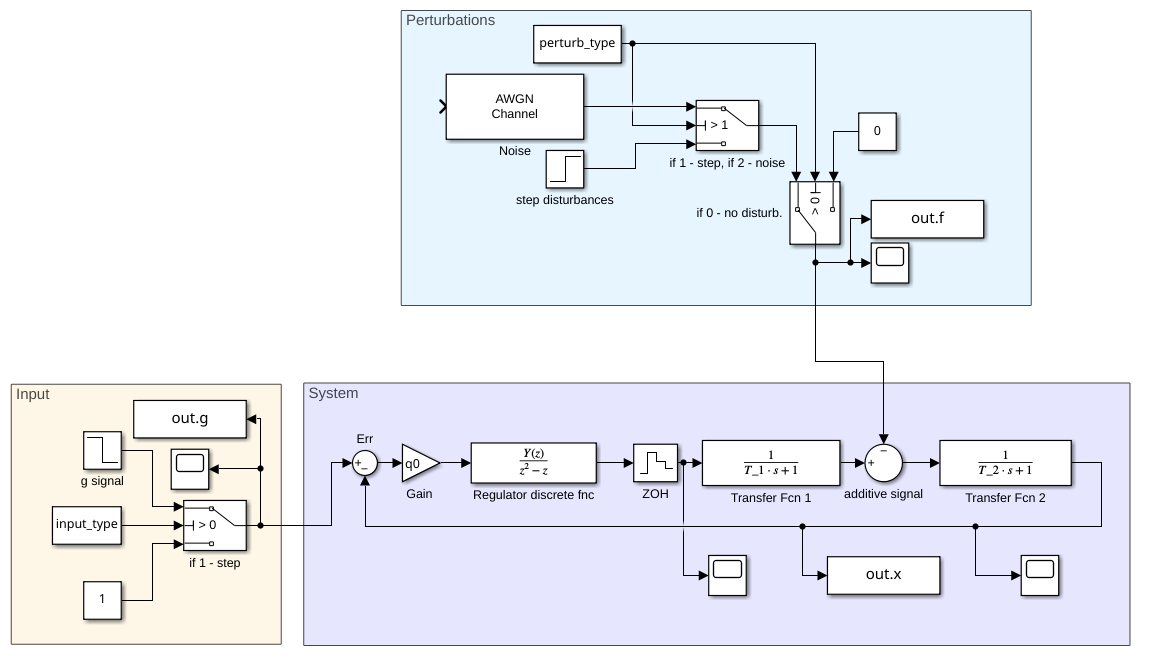
\includegraphics[width=\textwidth]{images/scheme.png}
    \caption{Схема.}
    \label{fig:scheme}
\end{figure}
В качестве параметров системы согласно варианту возьмем $T_1 = 0.85$, $T_2 = 0.95$.

\subsection{Подбор значения $q_0$}
Установим значение $T = \frac{T_1}{2}$. Проведем моделирование для различных значений $q_0$ при $g=1$, без внешних возмущений:
\begin{figure}
    [H]
    \centering
    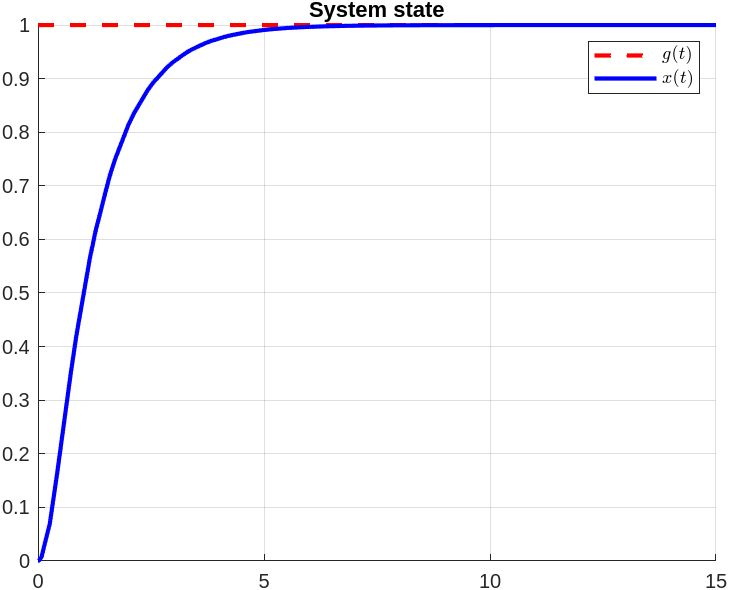
\includegraphics[width=300pt]{images/task2__q0_2_state.png}
    \caption{Задание 2. Моделирование при $q_0 = 2$.}
    \label{fig:task2__q0_2_state}
\end{figure}

\begin{figure}
    [H]
    \centering
    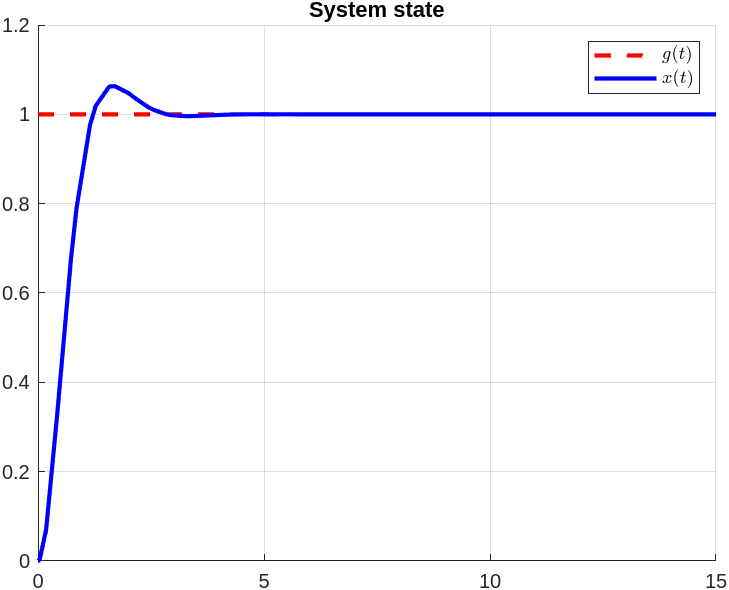
\includegraphics[width=300pt]{images/task2__q0_4_state.png}
    \caption{Задание 2. Моделирование при $q_0 = 4$.}
    \label{fig:task2__q0_4_state}
\end{figure}
\begin{figure}
    [H]
    \centering
    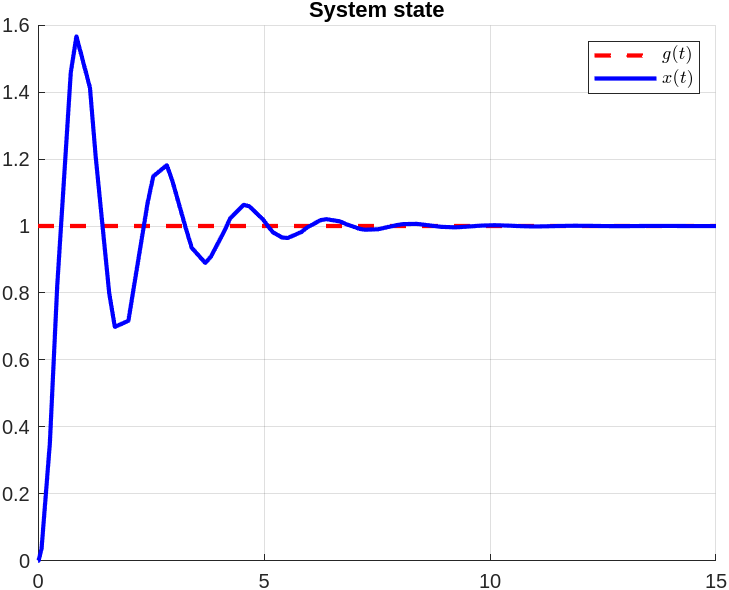
\includegraphics[width=300pt]{images/task2__q0_10_state.png}
    \caption{Задание 2. Моделирование при $q_0 = 10$.}
    \label{fig:task2__q0_10_state}
\end{figure}

Заметим, что при $q_0=4$  система имеет слабоколебательный переходный процесс.

\subsection{Исследование робастности системы}
Зафиксировав $q_0=$роведем моделирование системы при различных задающих воздействиях и внешних возмущениях:
\begin{figure}
    [H]
    \centering
    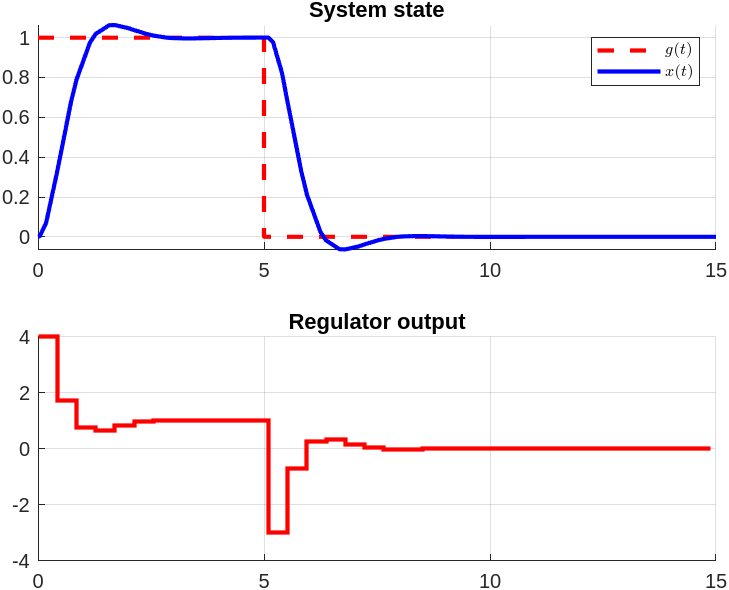
\includegraphics[width=300pt]{images/task3__step_input_state.png}
    \caption{Задание 3. Моделирование при ступенчатом изменении $g$, без возмущений.}
    \label{fig:task3__step_input_state}
\end{figure}
\begin{figure}
    [H]
    \centering
    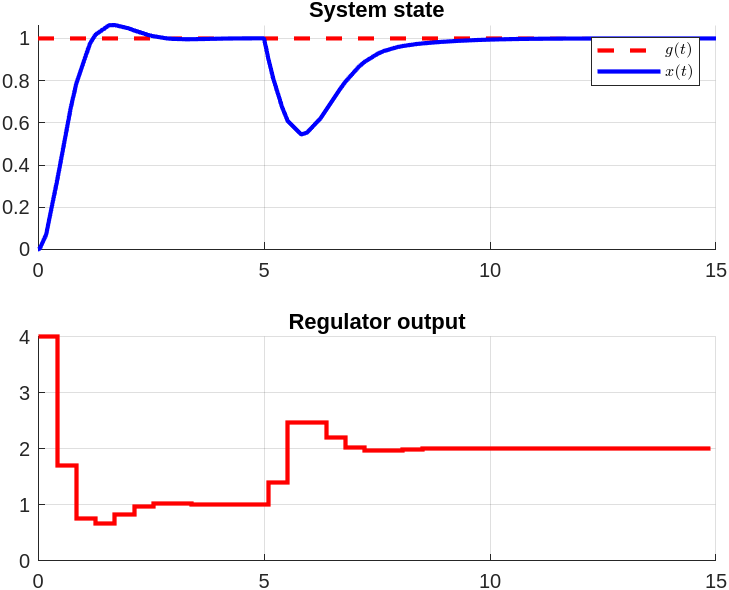
\includegraphics[width=300pt]{images/task3__step_perturb_state.png}
    \caption{Задание 3. Моделирование при $g=1$, ступенчатое изменение возмущений.}
    \label{fig:task3__step_perturb_state}
\end{figure}
\begin{figure}
    [H]
    \centering
    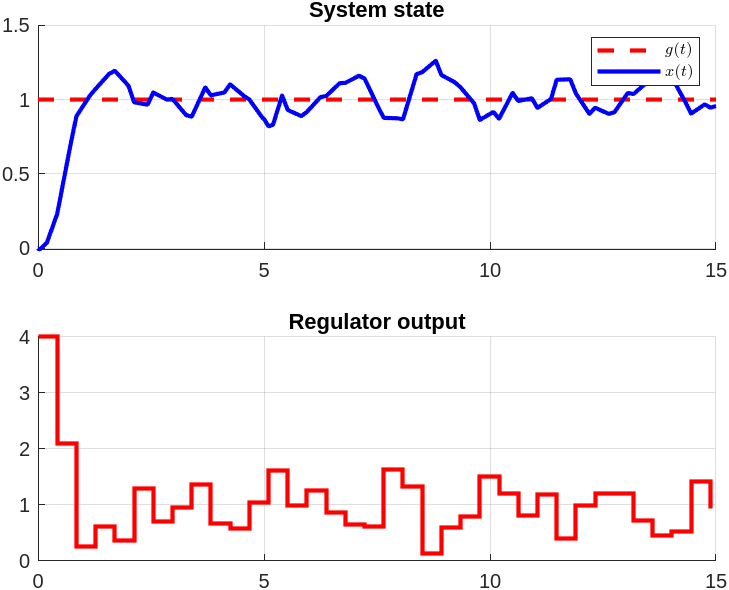
\includegraphics[width=300pt]{images/task3__noise_perturb_state.png}
    \caption{Задание 3. Моделирование при $g=1$, случайные возмущения.}
    \label{fig:task3__noise_perturb_state}
\end{figure}

Заметим, что система оказалась робастна в приведенных выше условиях эксперимента.
\subsection{Исследование влияния периода дискретизации}
Установим значение $T = \frac{T_1}{4}$. Проведем моделирование при ступенчатом изменении возмущения. Заметим, что колебательность исчезла:
\begin{figure}
    [H]
    \centering
    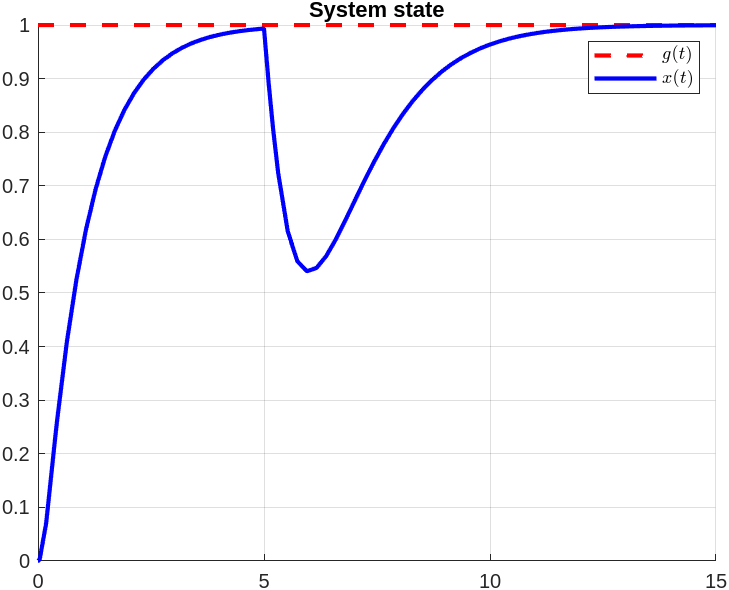
\includegraphics[width=300pt]{images/task4__step_perturb_state.png}
    \caption{Задание 4. Моделирование при $g=1$, ступенчатое изменение возмущений.}
    \label{fig:task4__step_perturb_state}
\end{figure}

\subsection{Исследование влияния неточности компенсации полюсов}
Проведем моделирование при увеличенном и уменьшенном значении $T_2$:
\begin{figure}
    [H]
    \centering
    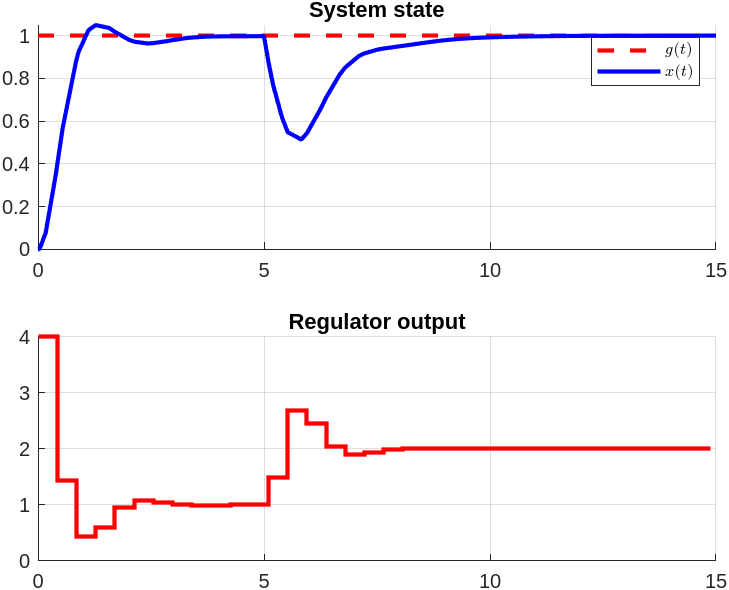
\includegraphics[width=300pt]{images/task5__decreased_state.png}
    \caption{Задание 5. Моделирование при уменьшенном значении $T_2$ ($80\%$).}
    \label{fig:task5__decreased_state}
\end{figure}
\begin{figure}
    [H]
    \centering
    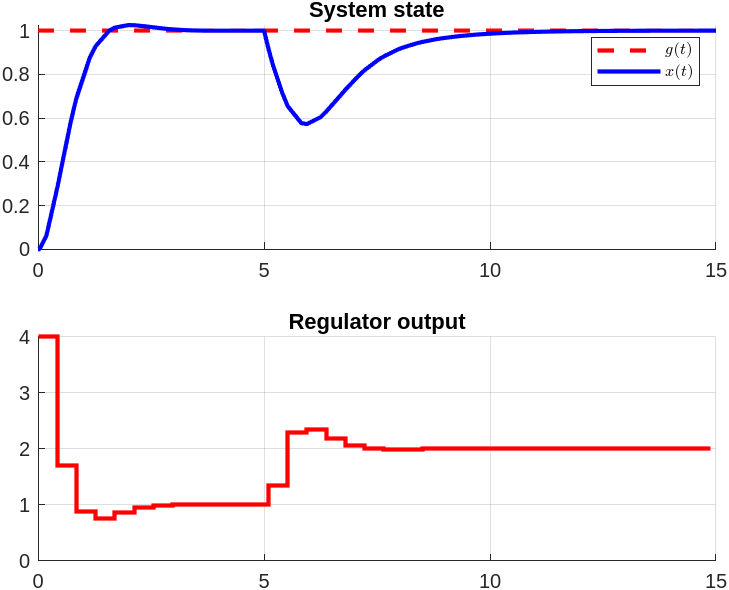
\includegraphics[width=300pt]{images/task5__increased_state.png}
    \caption{Задание 5. Моделирование при увеличенном значении $T_2$ ($120\%$).}
    \label{fig:task5__increased_state}
\end{figure}
Можем наблюдать усложнение динамики переходного процесса.

\section{Выводы}
В ходе выполнения лабораторной работы мы ознакомились с принципами синтеза ПИД-регулятора для дискретных систем. Можно выделить следующие замечания:
\begin{itemize}
	\item Изменение коэффициента $q_0$ влияет на полюса замкнутой системы, что позволяет настраивать поведение системы;
	\item При правильном выборе параметров регулятора замкнутая система робастна к ступенчатым изменениям задающего воздействия, а также возмущений;
	\item При наличии случайных возмущений система остается в окрестности устойчивого положения (однако важна частота изменения --- не должна сильно превышать $\frac{1}{T}$);
	\item Уменьшение интервала дискретизации увеличивает плавность переходных процессов и также оказывает влияние на полюса итоговой системы (в ходе эксперимента наблюдалось исчесновение слабоколебательного характера переходного процесса);
	\item При существовании неточности компенсации полюсов динамика замкнутой системы усложняется (за счет динамики изначальной), что может усложнить процесс настройки.
\end{itemize}

\end{document}